\documentclass{article}
\usepackage{graphicx}
\usepackage{amsmath, amssymb}
\usepackage{hyperref}

\title{Overall Survival Prediction for Patients Diagnosed with Myeloid Leukemia}
\author{Gaëtan Ecrepont}
\date{March 2025}

\begin{document}

\maketitle

\begin{abstract}
Predicting overall survival for patients diagnosed with myeloid leukemia is essential for personalized treatment. This report presents our approach using survival analysis techniques, in particular XGBoost, to model right-censored data effectively. We first introduce the problem and its challenges. When then describe our methodology and present our results. Finally, we discuss our model's limitations and ideas for improvement.
\end{abstract}

\section{Introduction}
Survival prediction is crucial in clinical settings to guide treatment decisions. However, the presence of right-censored data and a limited number of samples pose challenges. This study explores various survival analysis models and ultimately selects XGBoost for its performance and explainability.

\section{Problem Statement}
The dataset consists of clinical and genetic information, with the target variable being overall survival (OS). Key challenges include:
\begin{itemize}
    \item Right-censored data complicates standard regression techniques.
    \item Feature engineering is difficult due to domain-specific predictors.
    \item Missing data (7\% in clinical, 9\% in genetic data) requires imputation.
\end{itemize}

\section{Methodology}
We evaluated multiple models for survival prediction:
\begin{itemize}
    \item \textbf{Penalized Cox Model}: Simple and interpretable but lacks non-linearity.
    \item \textbf{Random Survival Forest}: Good interpretability but at risk of overfitting. Slow fit.
    \item \textbf{Kernel Survival SVM}: Performance heavily depends on the kernel choice. We weren't able to come up with a good enough kernel for this approach to be competitive. Besides, it lacks interpretability.
    \item \textbf{Survival XGBoost}: Gradient-Boosted Trees: high performance and fast training, but risk of overfit.
\end{itemize}
XGBoost was selected due to its superior performance and computational efficiency, though we had to tweak the hyperparameters to avoid overfitting.

\section{Feature Engineering}
\subsection{Clinical Features}
We first extracted information for the \texttt{CYTOGENETICS} column:
\begin{itemize}
    \item chromosomal anomalies: chromosome loss, gain, deletion, derivative, marker, short arm, long arm, translocation, XX, XY.
    \item missing cytogenetics.
    \item \texttt{n\_+-}: Total count of chromosome gains and losses.
    \item specific risk factors:  loss of chromosome 7, deletion of chromosome 5q, translocation between chromosomes 9 and 22.
    \item \texttt{cyto\_complexity}: Measure of karyotype complexity, defined as the count of commas in the cytogenetics.
    \item \texttt{n\_high \_risk\_markers}: Count of high-risk markers (found in the literature).
\end{itemize}

We also defined the following ratios:
\begin{itemize}
    \item \texttt{nlr}: Neutrophil-to-lymphocyte ratio.
    \item \texttt{plr}: Platelet-to-lymphocyte ratio.
    \item \texttt{blast\_wbc\_ratio}: Ratio of blast cells to white blood cells.
\end{itemize}

Finally we added the \texttt{IPSS\_R\_Score} (Revised International Prognostic Scoring System) as a feature, it is a well-known prognostic factor in myeloid leukemia, defined as the following linear combination:
\begin{equation}
    \texttt{IPSS\_R\_Score} = 0.4 \cdot \texttt{BM\_BLAST} - 0.3 \cdot \texttt{HB} - 0.2 \cdot \texttt{PLT} + 0.5 \cdot \texttt{cyto\_complexity}
\end{equation}

\subsection{Genetic Features}
We first grouped the genetic features by patients and created aggregates and counts. We then created the following features (one per patient):
\begin{itemize}
    \item \textbf{Gene statistics}: number of mutations, number of chromosome affected, number of genes affected, number of effects, and VAF (variant allele frequency) sum and max across the mutations.
    \item \textbf{Key genes}: flag for the presence of mutations in key genes (e.g., FLT3, NPM1, IDH1, IDH2, TP53, TET2, ASXL1, RUNX1, and DNMT3A).
    \item \textbf{Gene counts}: number of mutations in each gene.
    \item \textbf{Chromosome counts}: number of mutations in each chromosome.
\end{itemize}

\section{Experimental Setup}
\subsection{Data Transformation}
Although tree-based models do not care for data normalization, we still applied a transformation in the hope that it would help XGBoost find its splits. Besides, having Gaussian features was needed to test the penalized Cox model which is a linear model. We only transformed clinical features because they exhibited significant right skewness. We applied the Yeo-Johnson transformation to normalize the data. The Box-Johnson transformation was also considered, but since some variables could equal zero, it was not applicable.

\subsection{Data Imputation}
Missing values were imputed using two methods:
- \textbf{Clinical Dataset}: 7\% missing values. All real positive variables (blood counts and bone marrow blast percentage) were imputed using the mode. Missing cytogenetics were imputed with the string "missing" so that the model could know when a patient had no cytogenetics data available.
- \textbf{Genetic Dataset}: 9\% missing values. Missing values were first ignored when grouping by patients and creating aggregates and counts. Then those newly created variables were imputed using -1. This makes sense as almost all these variables are (nonnegative integer) counts or indicators, i.e. ordinal variables. For example, the number of mutations in a gene is a count variable, and the presence of a mutation is an indicator variable. The categorical -1 value indicates to the model that the patient has no data available for this variable. 

Empirically, other imputation methods (e.g., mean instead of mode, 0 instead of -1) did not yield significant differences in performance. We chose the above two approaches as they seemed most intuitive.

\subsection{Evaluation Metric}
Performance was assessed using IPCW-C-index, which is like the classic Concordance Index for Right Censored Data (C-index) but using inverse probability weighting to account for the right-censored nature of the data. A score of 0.5 indicates random predictions, while a score of 1.0 indicates perfect predictions (and a score of 0.0 indicates perfectly wrong predictions). Although complicated to compute, The IPCW-C-index is a robust metric for survival analysis.

\subsection{Cross-Validation}
We used 5-fold cross-validation to evaluate model performance. Note that to avoid data leakage, we performed the imputation the data transformation and imputation during the cross-validation process. We saw no use of Stratified K-Folds as the dataset was already balanced between dead and censored patients. Likewise, each patient had only one row so we did not need Group K-Folds.

\subsection{Hyperparameter Tuning}
XGBoost tuning is a delicate exercise. The large number of hyperparameters means that we can easily overfit the data, and yet one can obtain significant performance improvements by tuning them carefully. Since a full grid search would be too expensive and might lead to overfitting, we used a Bayesian optimization approach to find the best hyperparameters. We used the \texttt{optuna} library, which is a powerful and efficient hyperparameter optimization framework. The search space included:
\begin{itemize}
    \item \texttt{n\_estimators} $in [100, 500]$: Number of trees to be built.
    \item \texttt{learning\_rate} $in [0.001, 0.1]$: Step size shrinkage used in update to prevent overfitting.
    \item \texttt{max\_depth} $in [2, 6]$: Maximum depth of a tree.
    \item \texttt{subsample} $in [0.4, 0.8]$: Fraction of samples to be used for each tree.
    \item \texttt{colsample\_bytree} $in [0.4, 1.0]$: Fraction of features to be used for each tree.
    \item \texttt{colsample\_bylevel} $in [0.4, 1.0]$: Fraction of features to be used for each level.
    \item \texttt{colsample\_bynode} $in [0.4, 1.0]$: Fraction of features to be used for each node.
    \item \texttt{min_child\_weight} $in [1, 10]$: Minimum sum of instance weight (hessian) needed in a child.
    \item \texttt{gamma} $in [0, 5]$: Minimum loss reduction required to make a further partition on a leaf node.
\end{itemize}
Note that except for \texttt{n\_estimators}, all the other hyperparameters were added to combat overfit. Also, to have an idea of the degree of overfit for each hyperparameter configuration, we recorded the performance of the model on the training set while our search was optimizing performance on the test set.

\begin{itemize}
    \item \texttt{n\_estimators}: 369
    \item \texttt{max\_depth}: 3
    \item \texttt{learning\_rate}: 0.0197
    \item \texttt{subsample}: 0.432
    \item \texttt{colsample\_bytree}: 0.661
    \item \texttt{colsample\_bylevel}: 0.819
    \item \texttt{colsample\_bynode}: 0.413
    \item \texttt{min\_child\_weight}: 9
    \item \texttt{gamma}: 1.392
\end{itemize}

Note in particular the high \texttt{n\_estimators} to improve performance combined a small \texttt{max_depth} to limit overfitting.


\section{Results}
\subsection{C-IPCW scores}
Our XGBoost model had the following C-IPCW scores:
- \textbf{Local cross-validation score}: 0.726 test & 0.763 train, indicating a medium generalization gap.
- \textbf{Public leaderboard score}: 0.727, placing us 23rd.
- \textbf{Private leaderboard score}: 

\subsection{Feature Importance}
For more robustness, we used four different feature importance methods:
\begin{itemize}
    \item \textbf{Weight}: Total number of time a feature is used to split the data.
    \item \textbf{Total gain}: Total improvement in the loss function brought by a feature.
    \item \textbf{Total cover}: Total number of samples impacted by a feature across all splits.
    \item \textbf{Permutation importance}: Model-agnostic method that measures the increase in prediction error when a feature is randomly shuffled. This method is more robust to overfitting and provides a better estimate of feature importance, but it is also more computationally expensive.
\end{itemize}
Feature importance analysis showed that hemoglobin level (HB) was by far the most critical predictor, followed by (in no particular order of importance) BM\_BLAST, IPPS\_R\_Score, Cyto\_Complexity, and PLT. These are all clinical features and it makes sense that they matter more than genetic features since those are much less specific and thus their overall importance is lower (although for a given patient, they can be very important). The model also performed well on the training set, with a C-index of 76.2\%, so the generalization error is not too high.

For each method, we plotted the top 10 feature importance scores in Figure \ref{fig:feature_importance}. The first three plots show the built-in feature importance scores for the XGBoost model using different methods (weight, gain, and cover). The last plot shows the permutation importance scores, which provide a more robust estimate of feature importance. Note that in all plots, the most importance featue is HB, followed by BM\_BLAST, IPPS\_R\_Score, Cyto\_Complexity, and PLT in a more or less random order.

\begin{figure}[h]
    \centering
    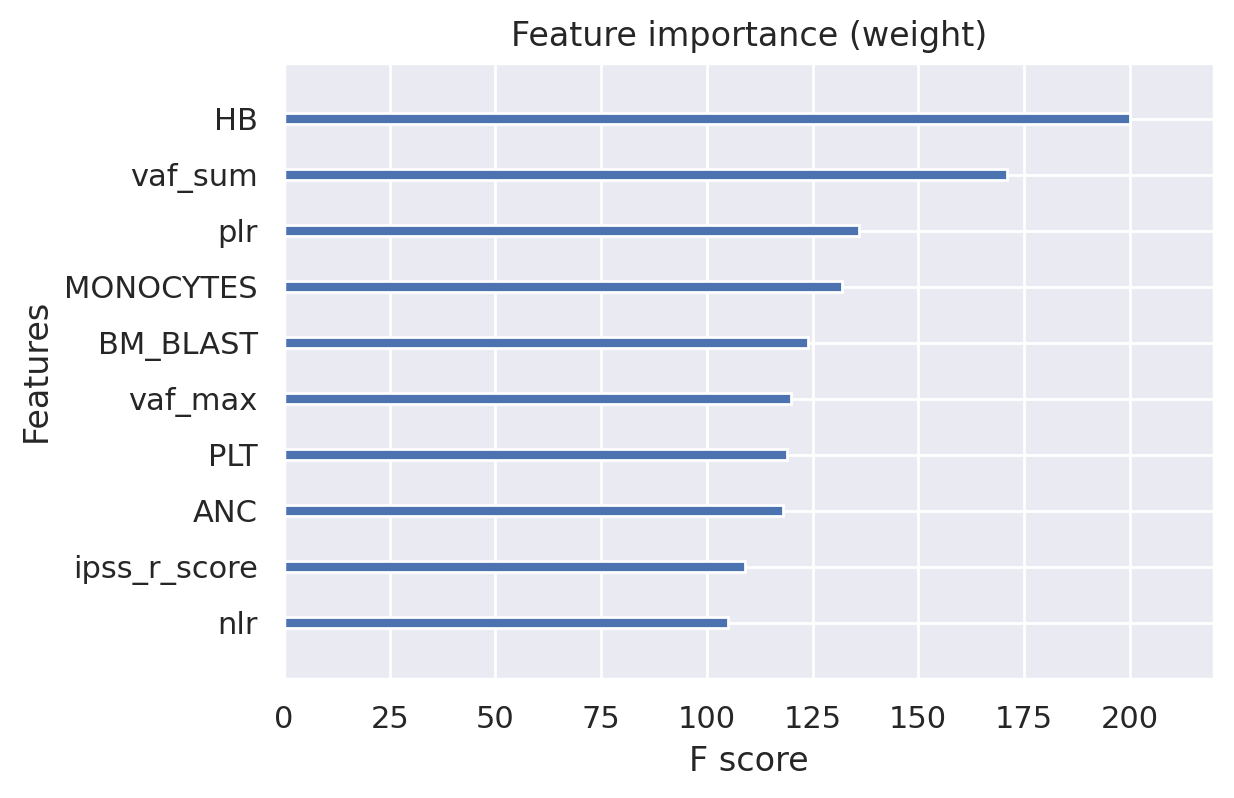
\includegraphics[width=0.6\textwidth]{img/feature_importance_xgb_weight.png}
    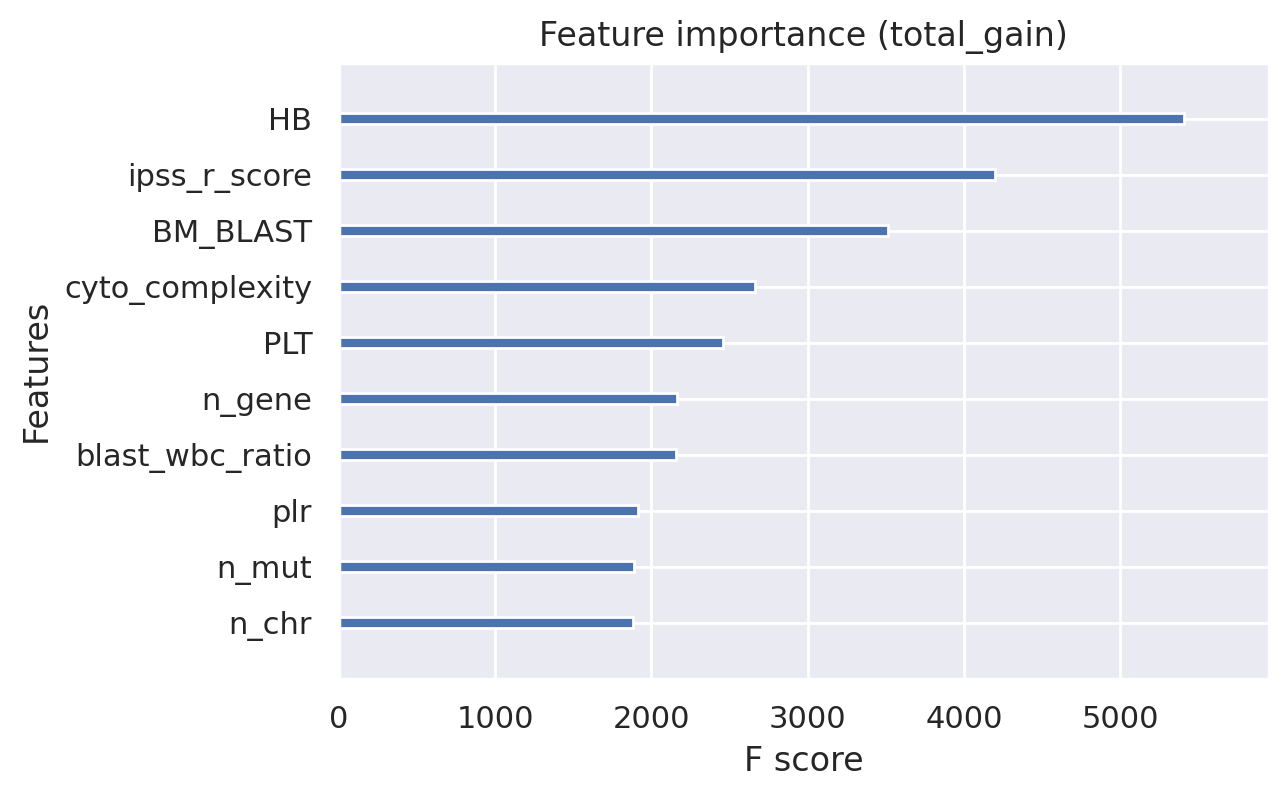
\includegraphics[width=0.6\textwidth]{img/feature_importance_xgb_total_gain.png}
    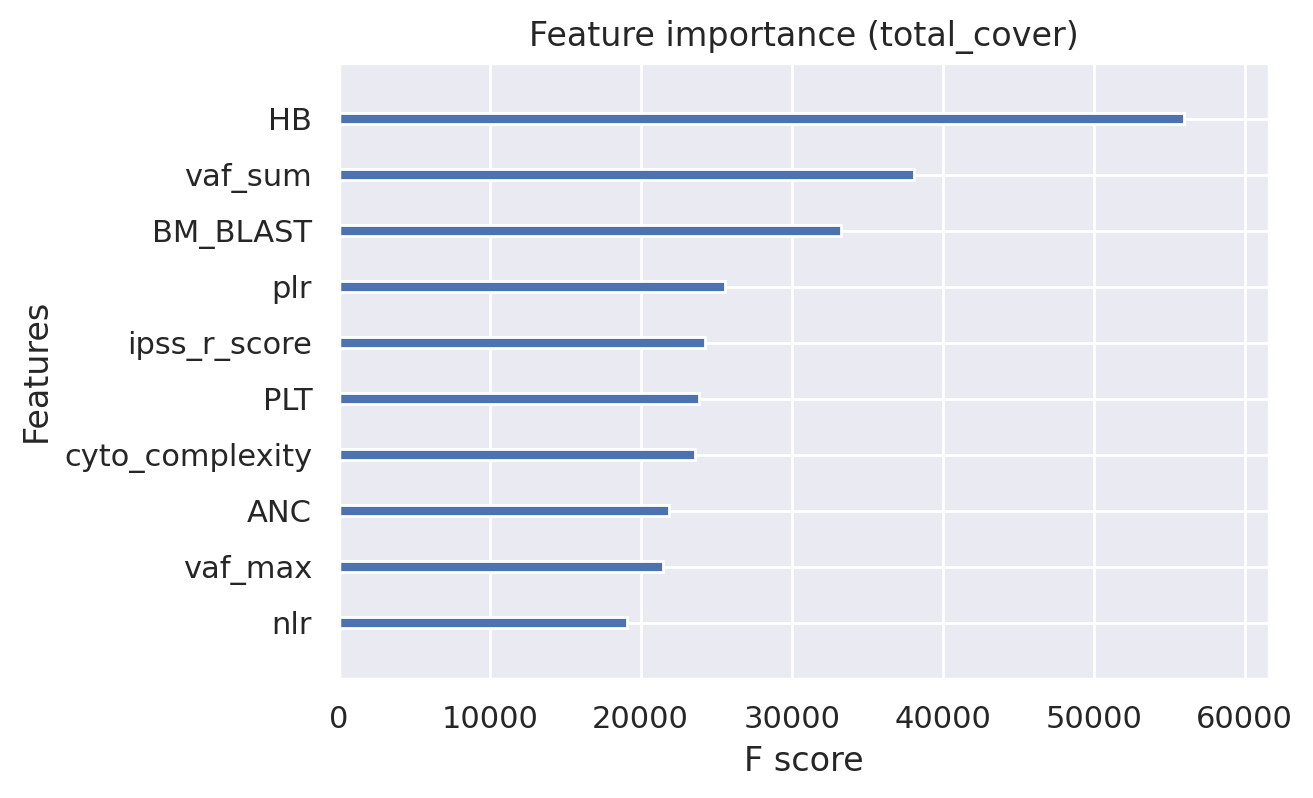
\includegraphics[width=0.6\textwidth]{img/feature_importance_xgb_total_cover.png}
    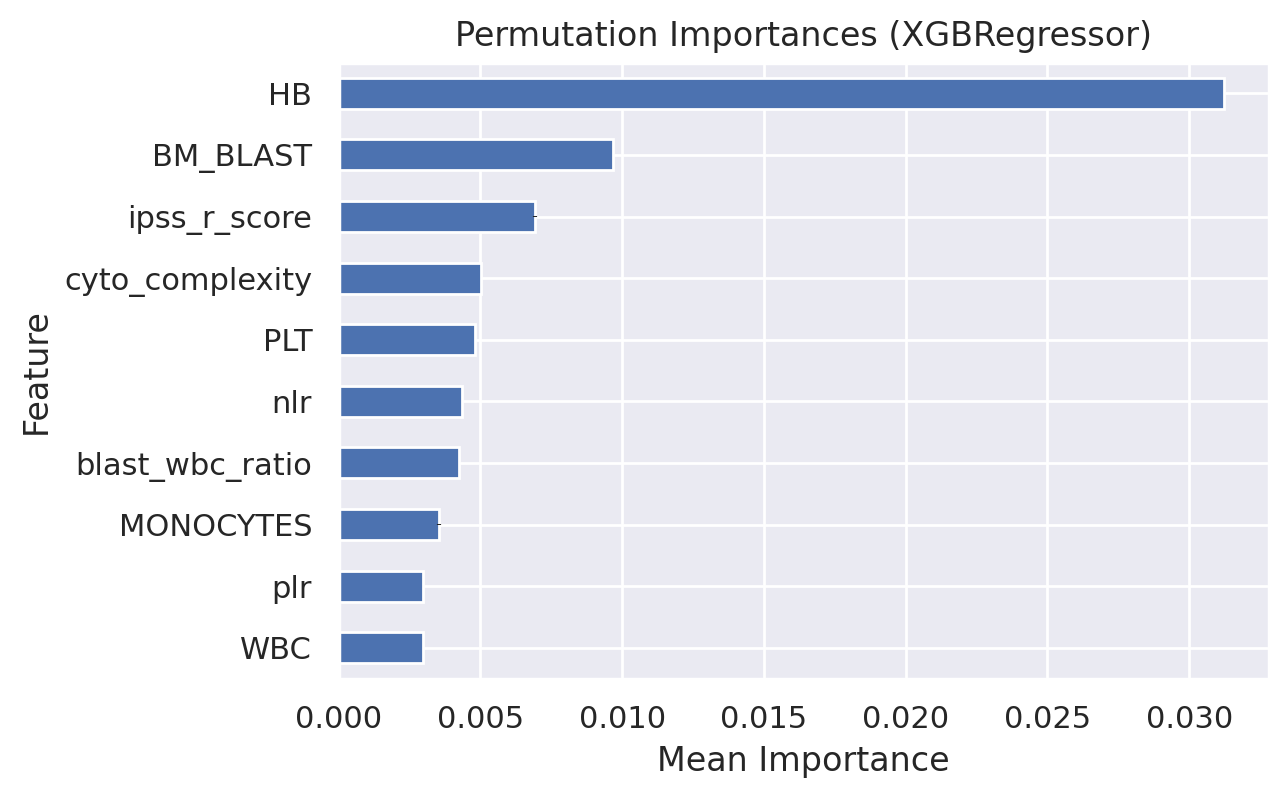
\includegraphics[width=0.6\textwidth]{img/permutation_importance_xgb.png}
    \caption{Feature importance scores for XGBoost model.}
    \label{fig:feature_importance}
\end{figure}


\subsection{Analysis of model performance}

The analysis of our model performance is not straightforward because the IPCW-C-index is complex. Since we are trying to predict the (relative) risk score of patients, one natural way to analyze the performance of our model is to look at how informative the risk score is. We can view this question using notions from classification, as if we were trying to predict whether the patient will die within the next 7 years\footnote{We censored observations at 7 years to compute C-IPCW.} or not.
\begin{itemize}
    \item \textbf{Precision}: When our model flags a patient as high-risk (resp. low-risk) does the patient indeed die within 7 years (resp. not die within 7 years)?
    \item \textbf{Recall}: When a patient dies (resp. doesn't die) within 7 years, does our model flag them as high-risk (resp. low-risk)?
    \item What happens in between?
\end{itemize}

To answer these questions, we can look at the scatter plot of the risk score against the actual survival time and survival class. The results are shown in Figure \ref{fig:precision_recall}. We find that the model has good precision for low-risk patients (blue oval) and high precision for high-risk patients (yellow oval). However, the model has medium recall for high-risk patients (purple oval). Finally, the model is globally quite uncertain for mid-risk patients (green oval). This is not surprising as the model is trying to predict a continuous variable (the risk score) and the outcome is binary (death of not).

To summarize our analysis: our model is good at flagging low-risk patients and high-risk patients, but it is moderately good at catching high-risk patients. Besides, our model globally behaves poorly outside the extremes: that is, our risk score is not very informative for mid-risk patients.

\begin{figure}[h]
    \centering
    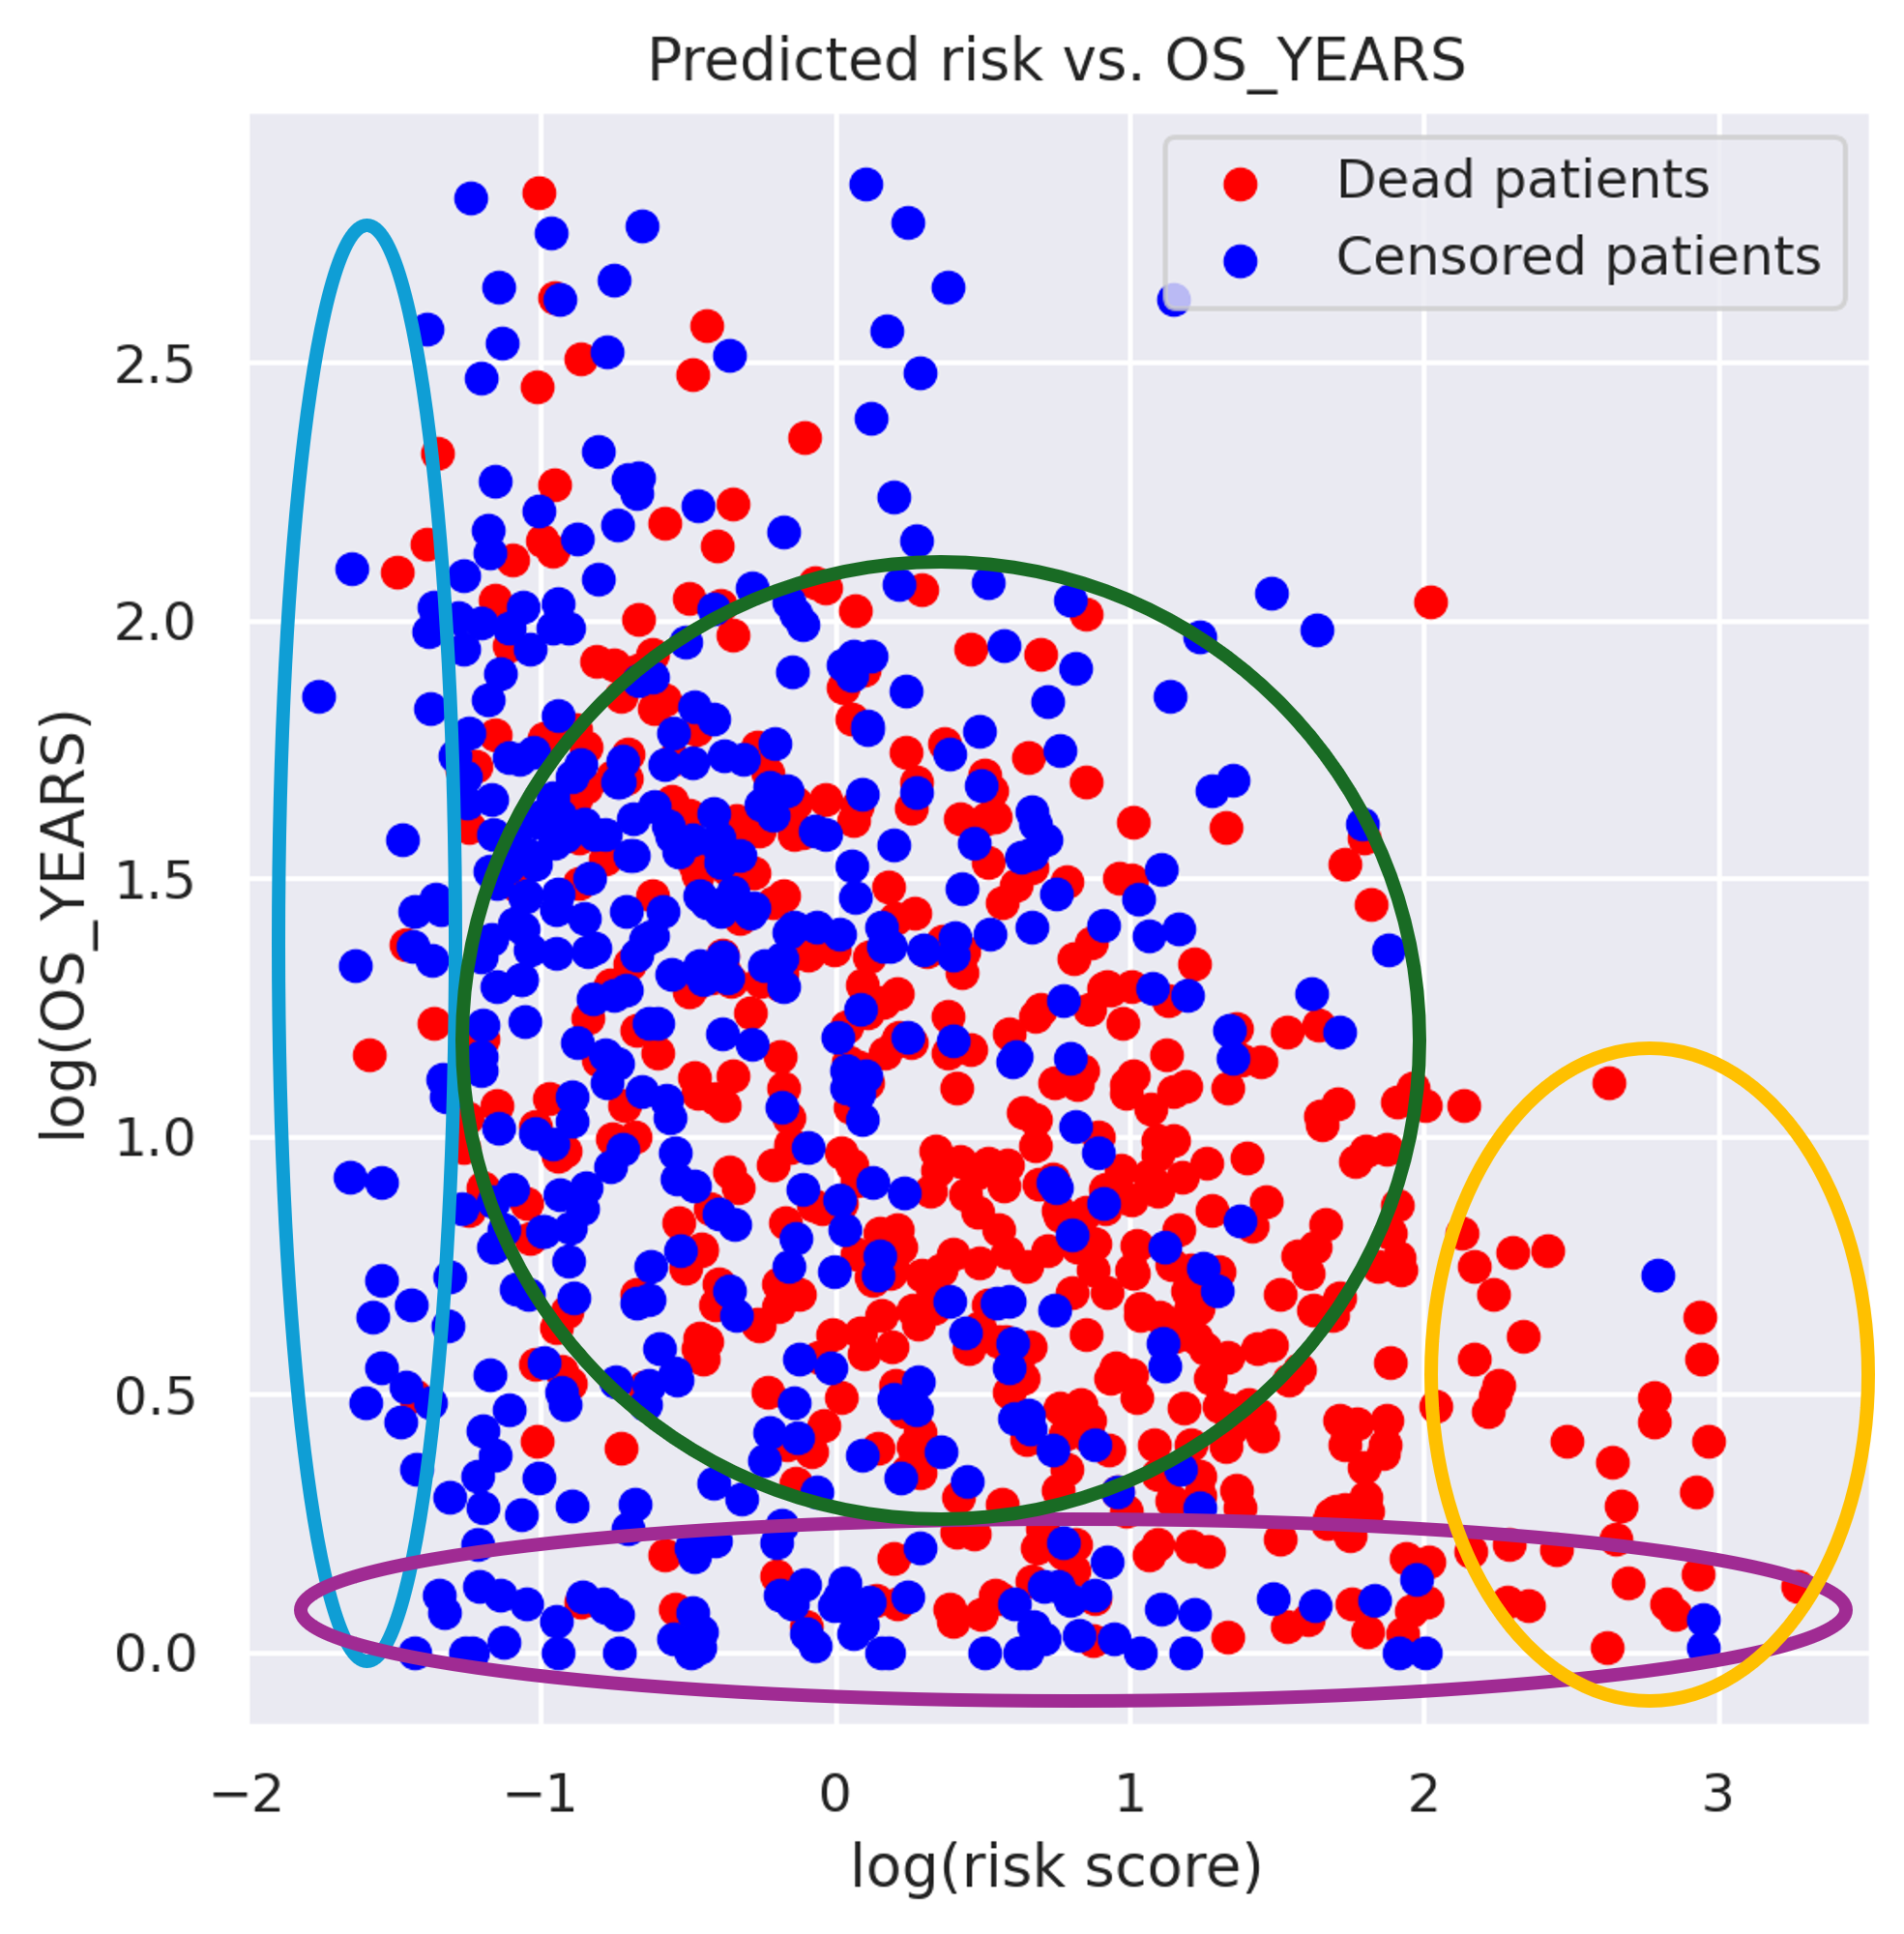
\includegraphics[width=0.8\textwidth]{img/risk_score_vs_OS_YEARS_annotated.png}
    \caption{Scatter plot of risk score against actual survival time, colored by survival class.}
    \label{fig:precision_recall}
\end{figure}


\section{Discussion}
While XGBoost performed well at identifying high- and low-risk patients, intermediate-risk predictions remained uncertain. Possible improvements include additional features, ensembling, and further hyperparameter tuning.

\section{Conclusion and Future Work}
This study demonstrated the potential of XGBoost for survival prediction in myeloid leukemia patients. Future work should focus on leveraging medical literature for feature engineering, ensembling different models, and refining hyperparameters.

\section{References}
\begin{thebibliography}{9}
    \bibitem{scikit-survival}
    Scikit-survival: A library for survival analysis in Python.
    \url{https://scikit-survival.readthedocs.io/en/stable/}
    
    \bibitem{optuna}
    Optuna: A hyperparameter optimization framework.
    \url{https://optuna.org/}

    \bibitem{XGBoost}
    XGBoost: A scalable tree boosting system.
    \url{https://xgboost.readthedocs.io/en/latest/}

    \bibitem{IPSS-R}  
    Revised international prognostic scoring system for myelodysplastic syndromes. *Blood*. 2012 Sep 20;120(12):2454-65. doi: 10.1182/blood-2012-03-420489. Epub 2012 Jun 27. PMID: 22740453; PMCID: PMC4425443.
    \url{https://pubmed.ncbi.nlm.nih.gov/22740453/}
\end{thebibliography}

\end{document}
